
% Chapter 2 File

\chapter{Introduction}
\label{chapter1}
\thispagestyle{empty}

% Retrons were first discovered in 1984 when researchers observed the "spontaneous" production of intracellular single-stranded DNA (ssDNA) in \textit{Myxococcus xanthus}, later identified as the product of an endogenous reverse transcriptase (RT) [1,2]. Over the past 35 years, studies on distinct retron systems have elucidated the mechanism behind RT-DNA production. However, their biological function remained largely unknown until recently. Today, we recognize retrons as tripartite bacterial defense systems composed of three components: a reverse transcriptase (RT), a non-coding RNA (ncRNA), and, in some cases, an effector protein or enzyme. These elements work together to protect bacteria against phage infections through a mechanism known as abortive infection, where the infected bacterial cell sacrifices itself to prevent viral replication, thereby safeguarding the bacterial population [3,4]. Currently, retrons not only help uncover molecular mechanisms to fight phage infections, but their unique features have also made them versatile tools with broad potential in biotechnology.

Retrons were first discovered in 1984 when researchers observed the
``spontaneous'' production of intracellular single-stranded DNA (ssDNA) in
\textit{Myxococcus xanthus}, later identified as the product of an endogenous
reverse transcriptase (RT) \cite{yee1984,lampson1989}. Over the past 35 years,
studies on distinct retron systems have elucidated the mechanism behind RT-DNA
production. However, their biological function remained largely unknown until
recently. Today, we recognize retrons as tripartite bacterial defense systems
composed of three components: a reverse transcriptase (RT), a non-coding RNA
(ncRNA), and, in some cases, an effector protein or enzyme. These elements work
together to protect bacteria against phage infections through a mechanism known
as abortive infection, where the infected bacterial cell sacrifices itself to
prevent viral replication, thereby safeguarding the bacterial population
\cite{millman2020,bobonis2022}. In this arrangement the ncRNA serves as both
template and scaffold: the DNA reverse transcribed from it remains attached to
its own template and, together with the RT, holds the effector inactive until
phage infection disrupts the complex \cite{wang2022,gao2020}.
\todo{cross check this sentence}
Because that
template region tolerates extensive sequence replacement, the same system can be
reprogrammed to produce user-defined ssDNA \textit{in vivo}
\cite{simon2019,khan2025}. Currently, retrons not only help uncover molecular
mechanisms to fight phage infections, but their unique features have also made
them versatile tools with broad potential in biotechnology.


% Retrons were first discovered in 1984 when researchers observed the
% ``spontaneous'' production of intracellular single-stranded DNA (ssDNA) in
% \textit{Myxococcus xanthus}, later identified as the product of an endogenous
% reverse transcriptase (RT) \cite{yee1984,lampson1989}. Over the past 35 years,
% studies on distinct retron systems have elucidated the mechanism behind RT-DNA
% production. However, their biological function remained largely unknown until
% recently. Today, we recognize retrons as tripartite bacterial defense systems
% composed of three components: a reverse transcriptase (RT), a non-coding RNA
% (ncRNA), and, in some cases, an effector protein or enzyme. These elements work
% together to protect bacteria against phage infections through a mechanism known
% as abortive infection, where the infected bacterial cell sacrifices itself to
% prevent viral replication, thereby safeguarding the bacterial population
% \cite{millman2020,bobonis2022}.

% At the heart of this system lies the ncRNA, which serves simultaneously as
% template and scaffold. The RT recognizes a conserved secondary structure formed
% by the \textit{msr}--\textit{msd} regions of the ncRNA and reverse transcribes
% the \textit{msd} region into a short, often highly structured ssDNA. The
% resulting RT-DNA remains covalently linked to the ncRNA through a
% 2$'$--5$'$ phosphodiester bond at a conserved branching guanosine, generating
% the branched RNA--DNA hybrid historically termed multicopy single-stranded DNA
% (msDNA) \cite{lampson1989,simon2019}. This hybrid is not antiviral by itself:
% together with the RT, it assembles into a complex that binds the effector and
% holds it in an inactive state \cite{wang2022}. Retrons therefore operate as
% guards rather than as direct sensors of the phage. Phage-encoded proteins that
% inhibit or modify host functions destabilize the complex, releasing the effector
% and unleashing activities such as NAD$^{+}$ depletion, membrane disruption or
% nucleotide hydrolysis, which arrest cellular metabolism before viral progeny can
% be assembled \cite{millman2020,bobonis2022,gao2020}.

% Notably, the very properties that make the ncRNA an effective scaffold in
% defense also make it an attractive substrate for engineering. The \textit{msd}
% region tolerates extensive sequence replacement and expansion without abolishing
% reverse transcription, so retrons can be reprogrammed to produce abundant,
% user-defined ssDNA \textit{in vivo} \cite{simon2019,khan2025}. Coupled with
% single-stranded annealing proteins or targeted nucleases, these
% retron-derived ssDNAs act as continuously regenerated donor templates for
% homologous recombination, enabling precise and massively parallel genome editing
% in bacteria, yeast and mammalian cells \cite{sharon2018,schubert2021,lopez2022}.
% Retrons thus occupy a dual position in current research: as a window into the
% molecular arms race between bacteria and phages, and as a modular platform for
% biotechnology.





\section{Retrons: Sequence and Structural Features}
\label{sec:features}

Although phage defense requires all three retron components, the reverse transcriptase (RT) and its cognate non-coding RNA (ncRNA) are sufficient to synthesize the single-stranded branched RNA–DNA complex, whereas the effector mediates the defense response itself \cite{simon2019,millman2020}. This functional modularity—specifically the ability to generate specific DNA sequences independently of host toxicity or defense pathways—underpins the utility of retrons as biotechnological tools. Accordingly, the following sections focus on the sequence and structural determinants of the RT and ncRNA, which directly dictate the yield, sequence identity, and length of the synthesized DNA.

\begin{figure}[H]
    \centering
    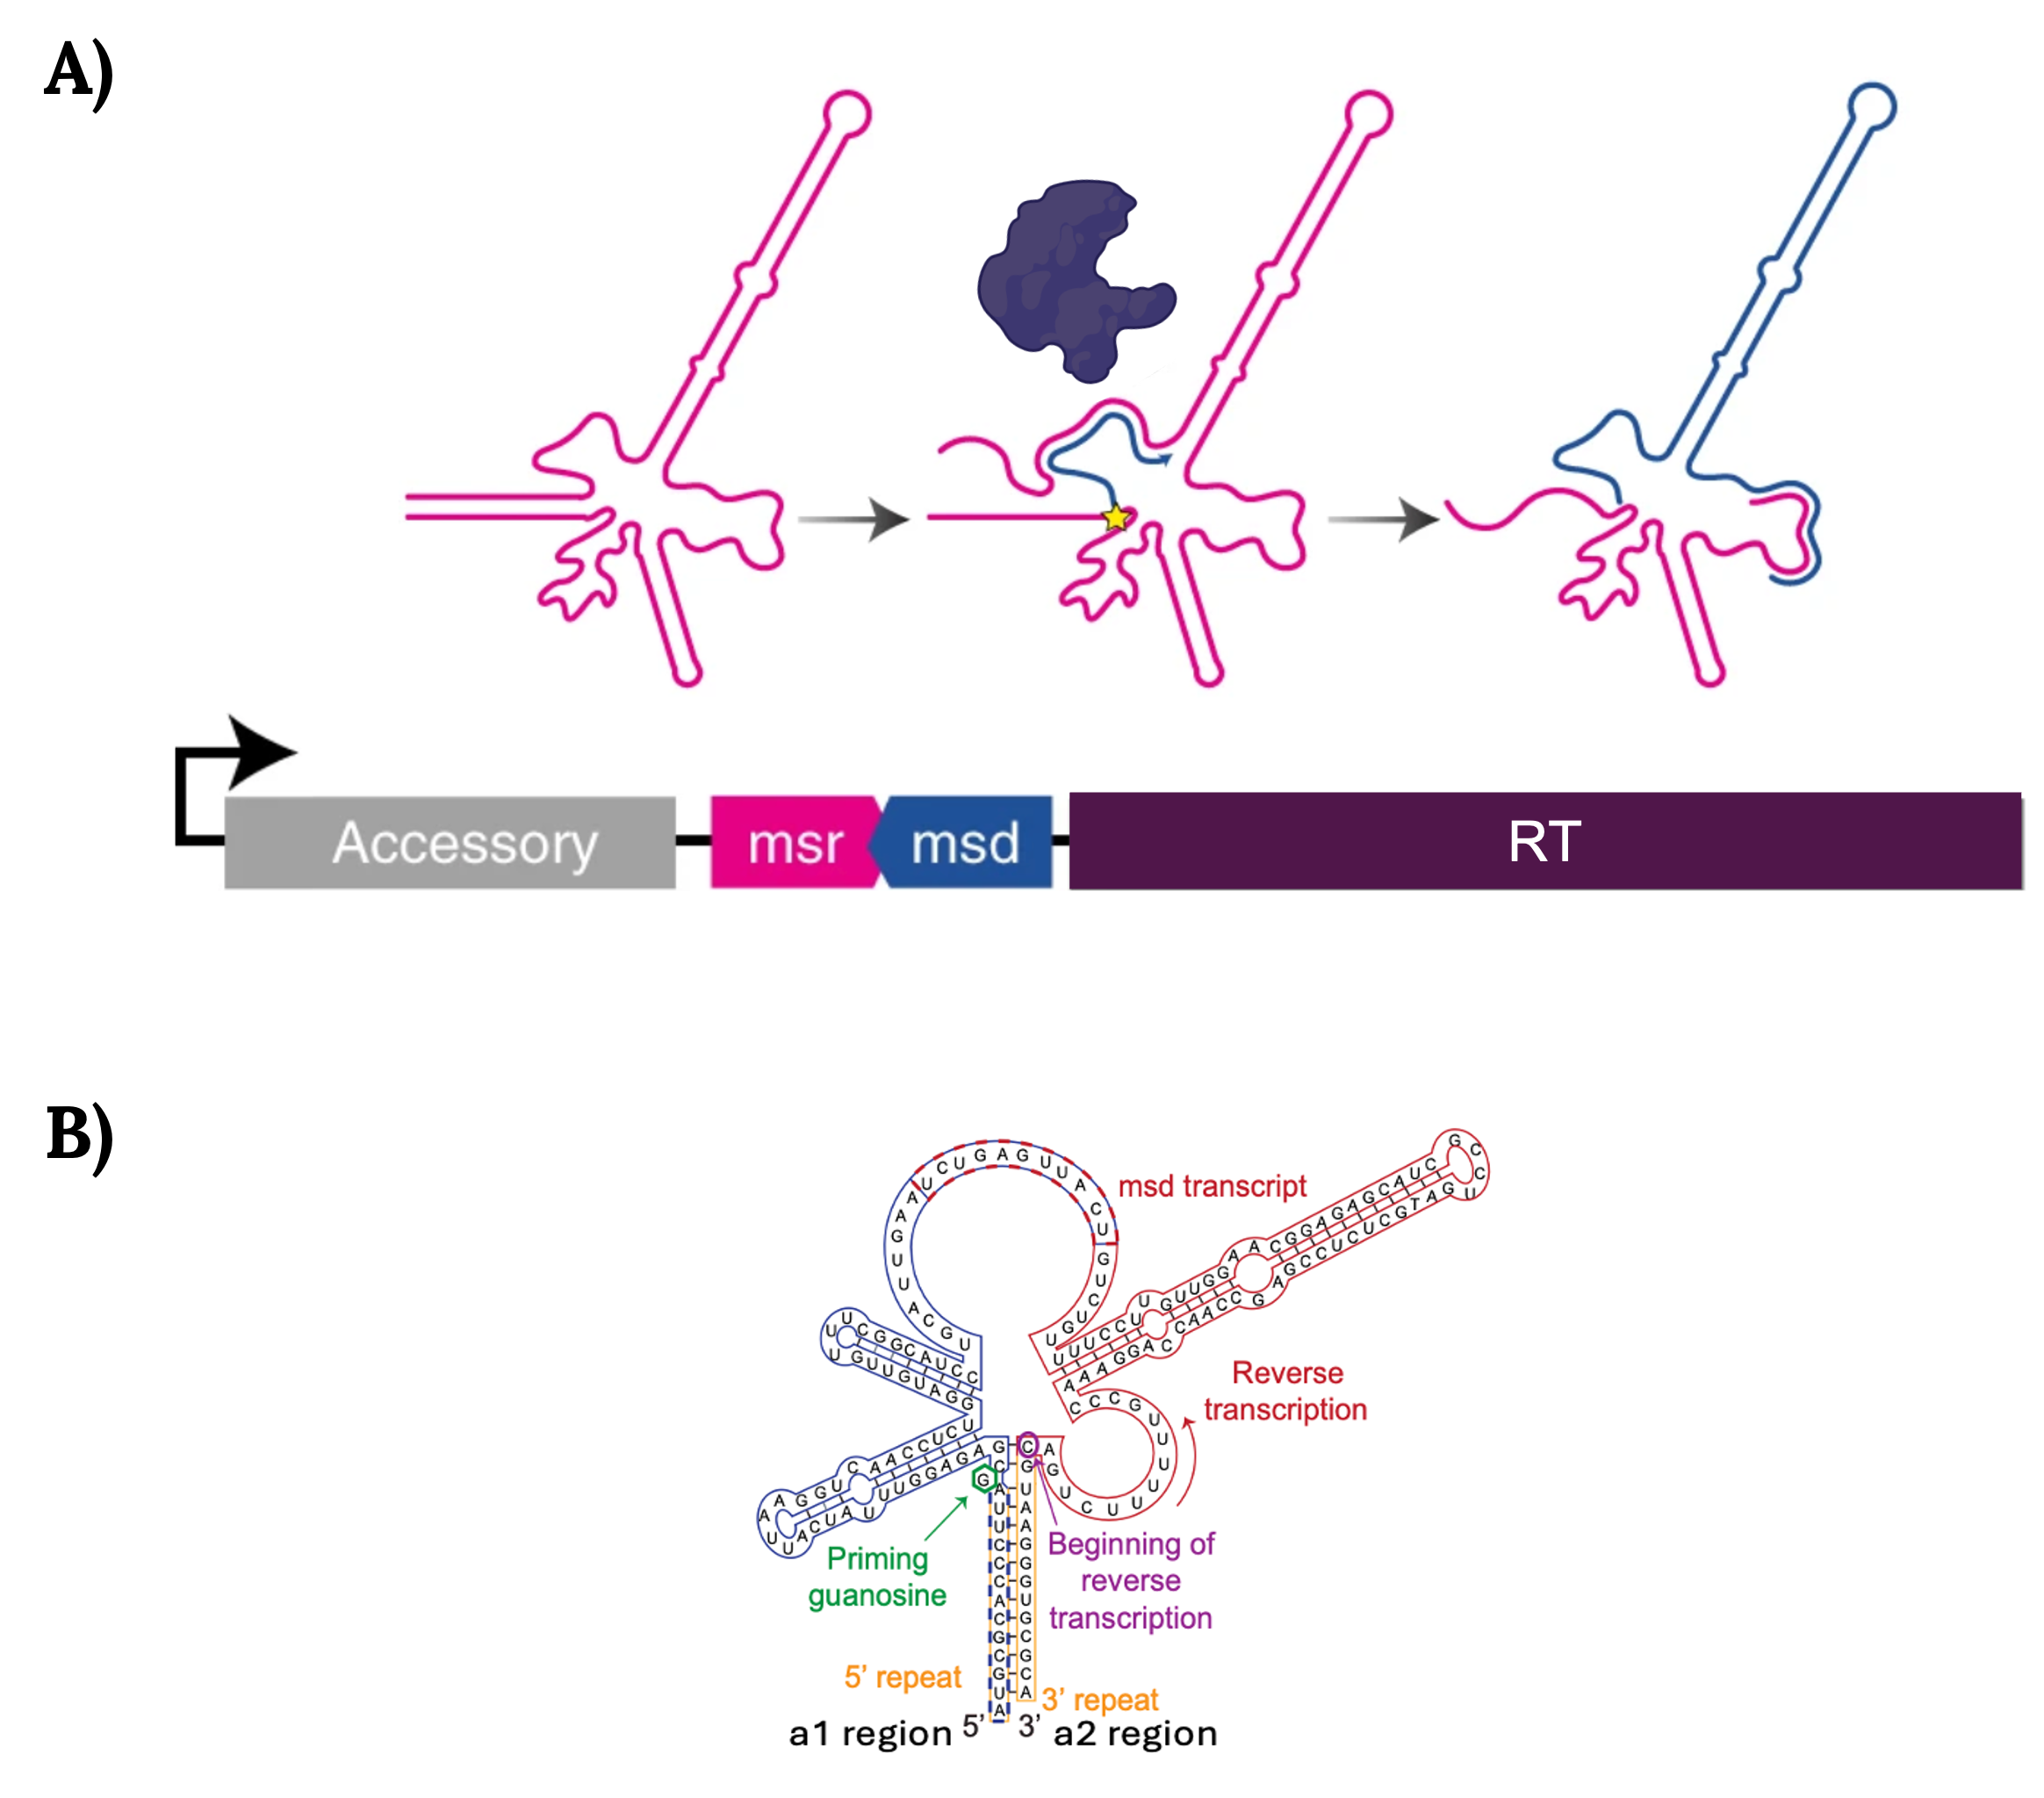
\includegraphics[width=0.75\textwidth]{retron_architecture.png}  % Adjust width as needed for smaller image
    \caption{Tripartite architecture of the retron operon organization and ncRNA architecture.}
    \label{fig:retron_architecture}
\end{figure}


\subsection{Architecture of the reverse transcriptase}
\label{sec:rt-architecture}

% https://claude.ai/chat/09520cf6-3c0b-45b7-a149-ce3906b70844

The reverse transcriptase (RT) at the core of retron systems displays a
characteristic right-hand-like fold consisting of finger, palm and thumb
subdomains. In the cryo-EM structure of Retron-Eco1 (Ec86), the L-shaped enzyme
is built from 13 $\alpha$-helices and 8 $\beta$-strands: the palm contributes a
four-stranded antiparallel $\beta$-sheet ($\beta$3--$\beta$6) packed against
$\alpha$5, $\alpha$9 and $\alpha$10, while the C-terminal thumb (approximately
residues 238--320) comprises a two-stranded antiparallel sheet
($\beta$7--$\beta$8) capped by a three-helix bundle ($\alpha$11--$\alpha$13)
\cite{wang2022}. The enzyme sits in a cavity of its own msDNA, held largely by
electrostatic complementarity between the nucleic-acid phosphate backbone and
the electropositive face of the protein, with the $3'$ ends of both chains close
to the active site \cite{wang2022}. Little else is present: retron RTs are
typically only 300--400 residues long and carry no bioinformatically detectable
endonuclease, maturase or RNase~H domain \cite{simon2019}, so template removal
falls to the host RNase~H1, which degrades the \textit{msd} template and also
influences where reverse transcription stops \cite{shimamoto1995,palka2022}.
Economical though it is, the fold is entirely conventional, superimposing well
on the RT domains of group~II intron maturase, HIV and telomerase reverse
transcriptases \cite{wang2022}.

This structural conservation is not matched at the sequence level. The seven
sequence blocks RT1--RT7 that are conserved across the RT superfamily are all
recognisable in Ec86 \cite{simon2019,wang2022}, and catalysis rests on the
familiar double-aspartate tetrad --- YADD in most retron RTs, a core shared with
group~II intron maturases and other bacterial RTs rather than diagnostic of
retrons, and not strictly invariant, since RT-Eco5 (Ec107) encodes YCDD
\cite{simon2019}. Outside these blocks, however, similarity falls away sharply.
The experimentally validated retron RTs share only $\sim$25\% average amino-acid
identity with one another, and just $\sim$14\% with the \textit{Roseburia
intestinalis} group~II intron maturase RT domain and $\sim$12\% with the
\textit{Bordetella} bacteriophage DGR RT \cite{simon2019}. Higher values are
confined to individual clades: RT-Sen2 (St85), RT-Eco4 (Ec83), RT-Eco7 (Ec78),
RT-Vch1 (Vc95) and RT-Vpa3 (Vp96) form a group whose members share
$\sim$40--58\% identity, and the two \textit{msr} pairs within it are similarly
close, which is why these are the only documented cases of an RT acting on a
non-cognate \textit{msr}--\textit{msd} \cite{simon2019}. Several retron RTs also
carry N- or C-terminal extensions of unknown function, most strikingly RT-Eco2
(Ec67) at 586 residues \cite{simon2019}.

Superimposed on the shared framework are two retron-specific regions.
Region~X is a segment of roughly 16 residues lying between RT2 and RT3 and
carrying a characteristic NAxxH motif, in which the histidine is the most
conserved residue; region~Y is larger, running some 90 residues from a conserved
VTG triplet within RT7 to the C-terminus, with the glycine most conserved
\cite{simon2019,mestre2020}. Region~X is diagnostic rather than merely present:
group~II intron and DGR RTs also carry residues between motifs~2 and~3, but
without the NAxxH signature \cite{simon2019}. Neither motif is invariant. Of the
sixteen experimentally validated retron RTs, fourteen carry NAxxH, the outliers
RT-Eco6 (Ec48) and RT-Mxa2 (Mx65) being substituted at the asparagine; fourteen
likewise carry VTG, with V$\rightarrow$I in RT-Vch2 (Vc81) and T$\rightarrow$H
in RT-Eco6 (Ec48) \cite{simon2019}. Both regions lie close to the catalytic
centre, consistent with a role in accommodating the $2'$-OH primer and the
branched product, and the functional evidence separates them cleanly. Deleting
region~X from RT-Eco1 (Ec86) or RT-Eco3 (Ec73) leaves cognate \textit{msr}
binding intact while abolishing DNA synthesis, placing its contribution at
initiation or catalysis rather than substrate recognition \cite{inouye1999};
deleting region~Y instead abolishes \textit{msr} binding, and swapping region~Y
between the two enzymes swaps their \textit{msr} specificity \cite{inouye1999}.
Consistently, an isolated C-terminal fragment of RT-Eco1 (residues 255--320)
binds the \textit{msr}-Eco1 stem-loop with $K_{\mathrm{D}} \approx
5\times10^{-8}$\,M but does not recognise \textit{msr}-Eco3 \cite{inouye2004}.
Region~Y is therefore the specificity determinant underlying the strict pairing
of each RT with its own ncRNA.

These interactions also organise the enzyme above the level of the monomer. In
Ec86, helix $\alpha$1 of one protomer packs against a surface of the second
together with nucleotides dA4, dG5 and dA6 of the \textit{msr}--msDNA hybrid;
truncating this helix compromises both msDNA production and phage defence, and
an N-terminal dimerisation helix of this kind is a recurring feature of type~II
retrons \cite{carabias2024,wang2026}. The resulting dimers stack into helical
filaments in which the msDNA scaffolds the assembly and cages the effector in a
low-activity state, so that shortening the msDNA disassembles the filament and
releases effector toxicity \cite{carabias2024}; an equivalent Ec86 filament is
triggered in cells by methylation of the msDNA by a phage-encoded cytosine
methyltransferase \cite{wang2024}. The same structures rationalise termination
of reverse transcription: the \textit{msr} segment 66--71, which connects the
\textit{msr}--msDNA duplex to the \textit{msr} hairpins, appears to displace the
$\beta$-hairpin carrying the fingers and so prevents coordination of the next
incoming nucleotide, and inserting extra nucleotides after A66 yields longer
msDNA products \cite{carabias2024}.



\begin{figure}[H]
    \centering
    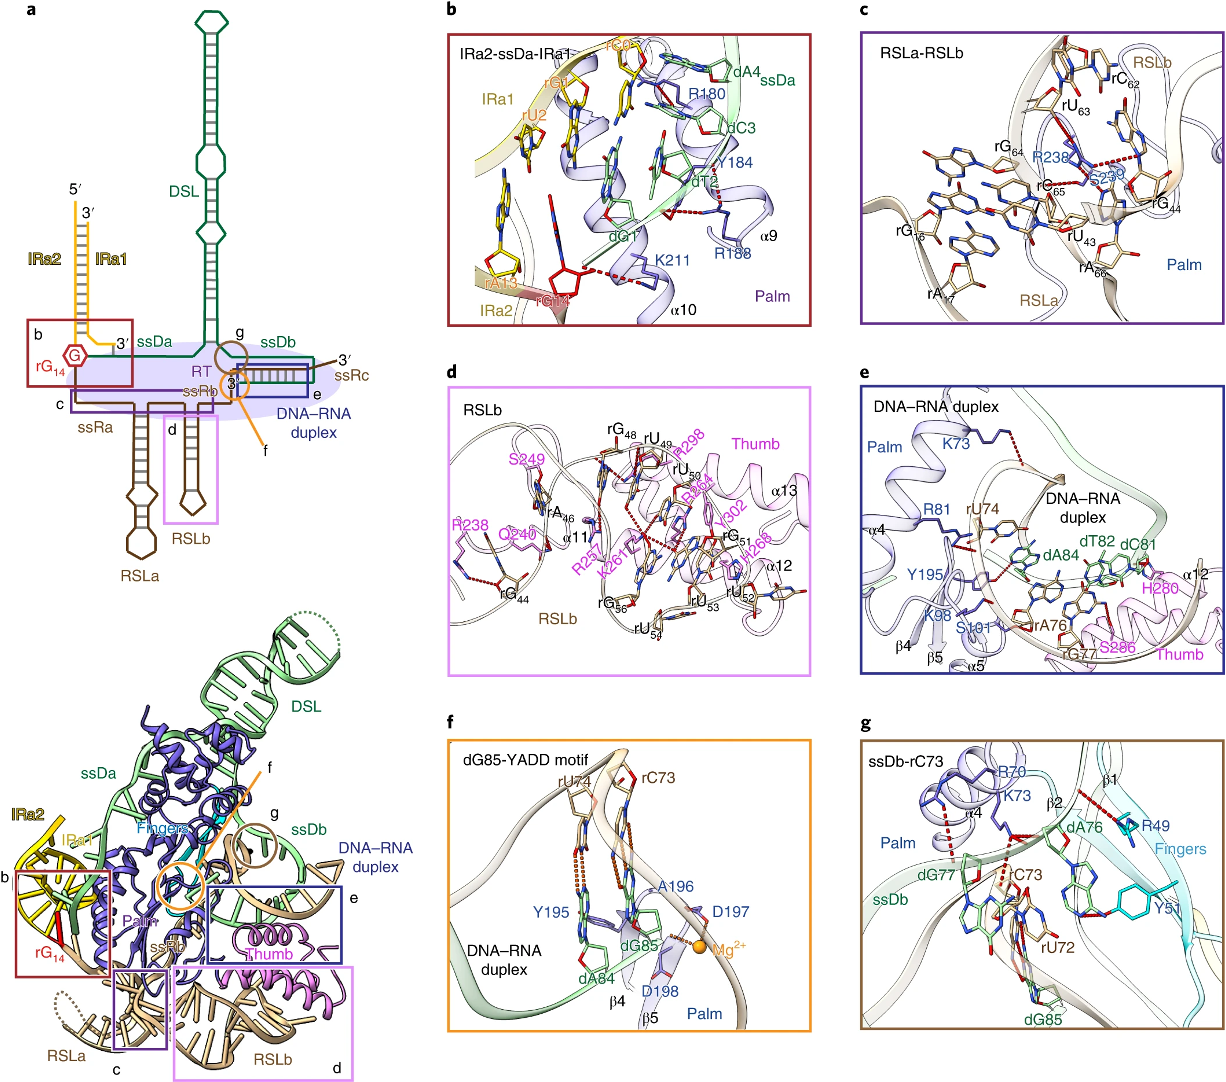
\includegraphics[width=1.0\textwidth]{ec86_structures.png}  % Adjust width as needed for smaller image
    \caption{TBD}
    \label{fig:Ec86_structure}
\end{figure}



% \caption{Architecture of the retron reverse transcriptase.
% (\textbf{a}) Alignment of representative retron RTs with a group~II intron
% maturase RT domain and the \textit{Bordetella} phage DGR RT. The seven universal
% RT blocks (RT1--RT7) are boxed in black and the retron-specific regions X and Y
% in red; the catalytic XXDD core is boxed in purple. Adapted from
% \cite{simon2019} under CC~BY~4.0. (\textbf{b}) Cartoon of RT-Eco1 (Ec86) bound to
% its msDNA, rendered from PDB~7XJG. Fingers, palm and thumb are coloured as in
% (\textbf{a}); msDNA is shown in grey. The YADD tetrad, N105/A106/H109 of
% region~X and V243/T244/G245 of region~Y are shown as sticks.}



% Two things to verify yourself: the shimamoto1993 page range (JBC 268, I have 2684–2692 but didn't confirm the last page), and crawford2025 first-author order. Also, if you want to note the exception to "msr always 5′ of msd," retron Se72 primes from a 3′ end and has an inverted arrangement — worth a sentence, but I'd let you pick the citation.



\subsection{Architecture and biogenesis of the retron ncRNA}

A retron minimally comprises a reverse transcriptase (RT) and a non-coding RNA
(ncRNA) transcribed as a single unit, together with, in most systems, associated
effector genes \cite{simon2019,mestre2020,millman2020}. The ncRNA carries two
functionally distinct regions: the \textit{msr}, retained as RNA in the mature
product, and the \textit{msd}, which templates DNA synthesis. The \textit{msr}
lies 5$'$ of the \textit{msd} in all experimentally validated systems
\cite{lampson1989,simon2019}. Primary sequence is poorly conserved between
families, whereas the predicted fold is not. Complementary segments at the 5$'$
and 3$'$ ends of the transcript (a1, a2) hybridise into a stem that closes the
molecule on itself and insulates the internal elements; a second internal pair of
inverted repeats (b1/b2) occurs in several systems \cite{mestre2020,simon2019}.
Within this scaffold the \textit{msr} is predicted to fold into one to three short
stem--loops with stems of 3--10\,bp, and the \textit{msd} into one or two long
hairpins whose stem is highly variable (10--50\,bp) and typically contains
mismatches and bulges \cite{mestre2020}.

This canonical description carries two caveats. First, it rests on thermodynamic
prediction and probing of the free transcript: 2$'$-hydroxyl acylation mapping of
the Retron-Eco1 ncRNA argues against several predicted internal hairpins, notably
the one proposed to enclose the termination site \cite{palka2022}. Second, the DNA
product need not retain its template's geometry --- in the cryo-EM structure of
Retron-Eco2 (Ec67) the reverse-transcribed strands hybridise into a DNA three-way
junction rather than the predicted stem--loop \cite{jasnauskaite2026}, although an
independent structure of the same complex did not resolve this junction
\cite{wang2025}. Predicted secondary structure is therefore best treated as a
model of the precursor, not of the mature particle.

Reverse transcription requires no separate primer. It initiates from the 2$'$-OH
of a conserved guanosine near the \textit{msr}--\textit{msd} boundary, often within
a TAGC motif, forming the 2$'$--5$'$ phosphodiester bond that tethers the nascent
DNA to its own template \cite{lampson1989,simon2019}; substituting this residue
abolishes priming \cite{hsu1992}. Synthesis proceeds toward the 5$'$ end of the
template and halts at a fixed position, giving each retron a product of
characteristic length --- the basis of the historical nomenclature, in which Ec86
(Retron-Eco1) denotes the \textit{E.~coli} retron producing an 86-nucleotide DNA
\cite{lampson1989,simon2019,millman2020}. In Retron-Eco2 (Ec67), priming occurs at
the branching residue G15 and synthesis stops at A67 \cite{lampson1989}.

Termination is imposed by nucleic-acid architecture rather than a sequence-encoded
stop signal. In the Retron-Eco1 filament, the fingers residues that would
coordinate an incoming nucleotide sit $\sim$9\,\AA{} from the catalytic centre in
an inactive configuration, the next templating base (U72) is held out of the pocket
by stacking against the nascent DNA, and \textit{msr} residues 66--71 appear to
displace the $\beta$-hairpin carrying the fingers; inserting nucleotides after A66
lengthens the product and compromises defence \cite{carabias2024}. In Retron-Eco2,
termination maps to the G52:dC67 base pair and involves flipping of the adjacent
template base U51 \cite{jasnauskaite2026}. Host factors also contribute: precise
termination in Retron-Eco1 additionally requires endogenous RNase H1, and loss of
\textit{rnhA} both lengthens the product and abolishes phage defence, suggesting
that template removal permits the tertiary DNA:RNA structure that enforces the stop
\cite{palka2022}. This requirement is not universal, as Retron-Eco2 is independent
of RNase H1 \cite{palka2022,jasnauskaite2026}. Because the stop is structural,
changing the \textit{msd} stem length changes the product length --- the property
exploited when retrons are retargeted \cite{lopez2022,crawford2025}.

Ribonucleolytic removal of the \textit{msd} template leaves the \textit{msr}
covalently attached through the 2$'$--5$'$ branch and base-paired to the 3$'$ end of
the DNA over a short duplex, so the mature msDNA is a covalent DNA--RNA chimera
rather than a free single strand \cite{palka2022,simon2019}. The maturating
nuclease is not uniform: RNase H1 fulfils this role in Retron-Eco1
\cite{palka2022}, whereas in Retron-Eco2 the RNase-H-like TOPRIM domain fused to
the RT is dispensable for biogenesis, implicating a different host enzyme
\cite{jasnauskaite2026}. Finally, retron RTs are specific for their cognate
ncRNAs: swapping \textit{msr}--\textit{msd} regions between retron-Ec67 and
retron-Ec73 abolishes msDNA production, whereas exchanging only the \textit{msr}
restores it, indicating recognition of both sequence and structure in the priming
region \cite{shimamoto1993}. An RT from one retron therefore generally cannot use
another's ncRNA, which constrains the modularity of engineered designs.


% https://claude.ai/chat/1f9cec06-7e54-45e7-b8c7-13ffe6a2e885

% A retron minimally comprises a reverse transcriptase (RT) and a non-coding RNA
% (ncRNA) transcribed as a single unit, together with, in most systems, one or more
% associated effector genes \cite{simon2019,mestre2020,millman2020}. The ncRNA
% carries two functionally distinct regions, \textit{msr} and \textit{msd}, with the
% \textit{msr} lying 5$'$ of the \textit{msd} in the experimentally validated
% systems \cite{lampson1989,simon2019}. The \textit{msr} is retained as RNA in the
% mature product; the \textit{msd} serves as the template that is copied into DNA.

% \subsubsection*{Predicted architecture of the precursor}

% Primary sequence is poorly conserved between retron families, whereas the
% predicted fold is comparatively well conserved. Short complementary segments at
% the 5$'$ and 3$'$ ends of the \textit{msr}--\textit{msd} transcript, a1 and a2,
% hybridise into a stem that closes the molecule on itself and places the internal
% elements in an insulated position; a second, internal pair of inverted repeats
% (b1/b2) has also been described in several systems
% \cite{mestre2020,simon2019}. Within this closed scaffold, comparative analysis of
% retron ncRNAs predicts that the \textit{msr} folds into one to three short
% stem--loops with stems of roughly 3--10\,bp, while the \textit{msd} folds into one
% or two long hairpins whose stem is highly variable, spanning about 10--50\,bp and
% typically containing mismatches and bulges \cite{mestre2020}.

% Two caveats attach to this canonical description. First, the folds above are
% largely inferred from thermodynamic prediction and from chemical probing of the
% free transcript. Selective 2$'$-hydroxyl acylation mapping of the Retron-Eco1
% ncRNA argues against several of the predicted internal hairpins, and specifically
% against the existence of the short hairpin that had been proposed to enclose the
% termination site \cite{palka2022}. Second, the DNA product need not retain the
% geometry predicted for its template. In the cryo-EM structure of Retron-Eco2
% (Ec67), the reverse-transcribed strands do not fold back as the predicted
% stem--loop but instead hybridise into a DNA three-way junction at the centre of
% the assembled trimer \cite{jasnauskaite2026}; notably, an independently determined
% structure of the same system did not resolve this junction \cite{wang2025}, so the
% point remains open. Predicted secondary structure should therefore be treated as a
% working model of the precursor rather than as a description of the mature
% particle.

% \subsubsection*{Priming, elongation and termination}

% Reverse transcription requires no separate primer. It initiates from the 2$'$-OH
% of a single conserved guanosine near the \textit{msr}--\textit{msd} boundary,
% frequently within a TAGC motif, generating the 2$'$--5$'$ phosphodiester bond that
% tethers the nascent DNA covalently to its own template
% \cite{lampson1989,simon2019}. Substitution of this residue abolishes priming
% \cite{hsu1992}. In Retron-Eco2 (Ec67) priming occurs at the branching residue G15
% of the primary transcript and synthesis stops at A67, yielding the 67-nucleotide
% DNA for which the retron was originally named \cite{lampson1989}. Synthesis
% proceeds toward the 5$'$ end of the template and halts at a fixed position rather
% than running to the end, so that each retron yields a product of characteristic
% length --- the basis of the historical nomenclature, in which Ec86 (Retron-Eco1)
% denotes the \textit{E.~coli} retron producing an 86-nucleotide DNA
% \cite{lampson1989,simon2019,millman2020}.

% Termination is imposed by the nucleic-acid architecture rather than by a
% sequence-encoded stop signal, and recent structures show how. In the Retron-Eco1
% filament, the fingers residues that would coordinate an incoming nucleotide sit
% roughly 9\,\AA{} from the catalytic centre in an inactive configuration, the next
% templating base (U72) is held out of the pocket by stacking against the nascent
% DNA, and the \textit{msr} segment spanning residues 66--71 appears to displace the
% $\beta$-hairpin that carries the fingers; inserting additional nucleotides after
% A66 lengthens the product and compromises defence \cite{carabias2024}. An
% equivalent arrangement is seen in Retron-Eco2, where termination maps to the
% G52:dC67 base pair and involves flipping of the adjacent template base U51
% \cite{jasnauskaite2026}. Host factors also contribute: in Retron-Eco1, precise
% termination requires endogenous RNase H1 in addition to the native ncRNA
% architecture, and loss of \textit{rnhA} both lengthens the product and abolishes
% phage defence, leading to a model in which removal of the RNA template permits the
% tertiary DNA:RNA structure that enforces the stop \cite{palka2022}. This
% requirement is not universal, since Retron-Eco2 produces its product independently
% of RNase H1 \cite{palka2022,jasnauskaite2026}. Because the stop is structural,
% altering the length of the \textit{msd} stem alters the length of the product,
% which is the property exploited when retrons are retargeted for DNA production and
% genome editing \cite{lopez2022,crawford2025}.

% \subsubsection*{Maturation and RT--ncRNA specificity}

% Cellular ribonuclease activity removes the \textit{msd} portion of the template
% after copying, leaving the \textit{msr} still covalently attached through the
% 2$'$--5$'$ branch and base-paired to the 3$'$ end of the DNA over a short duplex
% \cite{palka2022,simon2019}. The resulting msDNA is therefore a covalent DNA--RNA
% chimera rather than a free single strand, and it can undergo further nucleolytic
% processing in some systems. The identity of the maturating nuclease is not
% uniform: RNase H1 fulfils this role in Retron-Eco1 \cite{palka2022}, whereas in
% Retron-Eco2 the RNase-H-like TOPRIM domain fused to the RT is dispensable for
% msDNA biogenesis, implicating a different host ribonuclease
% \cite{jasnauskaite2026}. Finally, retron RTs are highly specific for their cognate
% ncRNAs. Swapping \textit{msr}--\textit{msd} regions between retron-Ec67 and
% retron-Ec73 abolishes msDNA production, whereas exchanging only the \textit{msr}
% restores it, indicating that recognition depends on both primary sequence and
% secondary structure of the priming region \cite{shimamoto1993}. This specificity
% explains why an RT from one retron generally cannot use the ncRNA of another, and
% it constrains the modularity available to engineered designs.


% The reverse transcriptase (RT) at the core of retron systems displays a characteristic right-hand-like fold consisting of finger, palm, and thumb subdomains. Cryo-EM structures of the Escherichia coli Ec86 retron revealed that the RT contains 13 α-helices and 8 β-strands, with the palm domain forming a 4-stranded antiparallel β-sheet flanked by α-helices, while the thumb domain contains a 2-stranded antiparallel β-sheet followed by a 3-helix bundle [18]. The RT possesses seven universal regions that align with other reverse transcriptases, including the highly conserved catalytic core YADD (Tyr-Ala-Asp-Asp) motif located in the palm domain. Additionally, retron RTs contain two specific regions, designated X and Y, with conserved amino acid sequences NAxxH and VTG, respectively, positioned close to the catalytic site [18]. Structural studies of Retron-Eco1 have provided insights into the RT's termination mechanism, revealing that specific conformational features of the msr-msDNA hybrid prevent the next nucleotide from entering the catalytic pocket, with the msr region 66-71 displacing the β hairpin carrying the fingers domain [17]. In the functional retron complex, the RT sits in a cavity formed by the msDNA, with interactions primarily mediated through the negatively charged phosphate backbone of msDNA and the RT's electropositive surface [Wang et al., 2022]. Retron RTs exhibit strong co-evolutionary relationships with their associated proteins and ncRNAs, suggesting mutual selective pressure and continuous evolution of the tripartite system [16]. In some retron systems, the RT forms filamentous assemblies with the effector protein, with the msDNA stem-loops arranged in a staggered configuration that scaffolds effector dimers, a structure essential for phage defense [17] These structural features enable the precise recognition and processing of the ncRNA template, which is fundamental to the retron's molecular mechanism.
% Retrons employ a distinctive molecular mechanism to produce msDNA (multicopy single-stranded DNA). The system consists of a reverse transcriptase (RT) and a non-coding RNA (ncRNA) that contains two key regions: msr (RNA portion) and msd (template for DNA synthesis) [13, 14]. 


% \\


% The ncRNA adopts a conserved secondary structure critical for function, where complementary sequences at the 5' and 3' ends (a1 and a2 regions) hybridize to form a double-stranded stem, insulating the internal structures [3, 14, 15]. The msr region typically forms 1-3 short stem-loops of 3-10 bp, while the msd region folds into a long hairpin with a highly variable stem of 10-50 bp [ 6, 14]. Reverse transcription initiates from a conserved guanosine residue, often found within a TAGC sequence motif, located near the junction of the msr and msd regions [6, 13, 15]. This guanosine's 2'-OH group serves as a primer, resulting in the formation of a unique 2'-5' phosphodiester linkage between the RNA template and the nascent DNA strand [3, 6, 13]. As the RT synthesizes DNA toward the 5' end of the template, it terminates at a defined position through an RNA structure-dependent mechanism [6]. Concurrently, cellular RNase H degrades most of the RNA template strand, except for approximately 5-10 nucleotides at the 5' end that remain hybridized to the complementary DNA [3, 6]. The resulting msDNA, a single-stranded DNA/RNA chimeric molecule, can undergo further nucleolytic processing to generate its mature form [6]. Importantly, retron RTs exhibit high specificity for their cognate ncRNAs, recognizing both sequence elements and secondary structure features, which explains why RTs from one retron typically cannot utilize the ncRNA from another [6].


% \section{Retrons as tools in Biotechnological Applications}

% Retrons have emerged as versatile molecular tools with applications extending beyond their original characterization as bacterial defense systems. Their ability to generate single-stranded DNA \textit{in vivo} through reverse transcription provides a programmable source of intracellular DNA that can be coupled to genome engineering, molecular recording, biosensing, and continuous-evolution platforms. Selected examples of these applications and their underlying mechanisms are summarized in Table~\ref{tab:retron_biotechnological_applications}. Strikingly, however, these diverse biotechnological applications have been developed from a remarkably limited number of experimentally validated retron systems \cite{simon2019}. This suggests that the current application landscape likely represents only a small fraction of the functional potential encoded within naturally occurring retron diversity.

% \\

% The engineering-relevant consequence of the above is a division of labour within
% the ncRNA between a recognition module that is read by the RT and a cargo module
% that is merely copied. Systematic mutagenesis of the Retron-Eco1 ncRNA supports
% this. Single-nucleotide substitutions are broadly tolerated except around the
% priming guanosine and the putative RT recognition loop in the \textit{msr};
% deletions are tolerated far less well, particularly in the \textit{msr} stem--
% loops and immediately flanking a2, indicating that structure matters more than
% sequence in these regions. The \textit{msd} hairpin, by contrast, accepts
% extensive substitution, and extension of the a1/a2 stem raises production
% \cite{crawford2025}. The permissiveness of the \textit{msd} is what makes the
% ncRNA a programmable object, and the intolerance of the \textit{msr} and a1/a2
% sets the boundary of that programmability. The choice of scaffold remains an
% experimental variable in its own right: across more than a hundred previously
% untested natural retrons, RT-DNA yield varies by orders of magnitude and the
% sequence of the product could not be predicted from the retron sequence alone
% in a substantial fraction of cases \cite{khan2025}.

% \\

% % A major expansion of this experimental foundation was provided by Shipman \textit{et al.}, who increased the number of experimentally validated retrons from the small set previously available to roughly 160 systems: : 62 of 98 newly tested retrons produced
% % detectable RT-DNA in \textit{Escherichia coli}, 29 were tested for
% % recombineering of the \textit{E.~coli} chromosome and 18 for the phage $\lambda$
% % genome, and of 140 constructs assayed in human HEK293T cells, , 101 produced
% % precise edits and 58 outperformed the standard retron-Eco1. 
% A major expansion of this foundation was provided by Khan \textit{et al.}
% \cite{khan2025}. Sampling every RT clade of the Rodr\'iguez Mestre
% classification, they synthesised 163 reverse transcriptases with their cognate
% ncRNAs and assayed them across contexts: 62 of 98 newly tested retrons produced
% detectable RT-DNA in \textit{Escherichia coli}, 29 were tested for
% recombineering of the \textit{E.~coli} chromosome and 18 for the phage $\lambda$
% genome, and of 140 constructs assayed in human HEK293T cells, 101 produced
% precise edits and 58 outperformed the standard retron-Eco1. These phenotypes
% track the classification of Rodr\'iguez Mestre \textit{et al.}
% \cite{mestre2020}, varying significantly by RT clade and, within productive
% clades, by retron subtype. Prediction nonetheless remains limited, as the
% sequence of each RT-DNA still had to be determined empirically.

% \\

% This expansion is particularly important because retron-based technologies generally require optimization or engineering of the retron components, including the ncRNA that encodes the ssDNA product and the cognate reverse transcriptase. Consequently, increasing the diversity of experimentally characterized retrons provides not only additional systems for biotechnology, but also a broader sequence and functional space from which general design principles can be established. In this direction, subsequent work using machine learning and large-scale Retron-Eco1 ncRNA variant libraries demonstrated that sequence-based models can identify ncRNA variants that maintain or improve reverse-transcription efficiency. 

% Together, the expansion of the retron repertoire and the development of systematic engineering approaches provide a foundation for exploring retron functions beyond those represented by the currently established applications, potentially unlocking new molecular recording, genome engineering, and biosensing capabilities.


\section{Retrons as tools in Biotechnological Applications}

Retrons have emerged as versatile molecular tools with applications extending
beyond their original characterisation as bacterial defence systems. Their
ability to generate single-stranded DNA \textit{in vivo} through reverse
transcription provides a programmable source of intracellular DNA that can be
coupled to genome engineering, molecular recording, biosensing and
continuous-evolution platforms. Selected examples of these applications and
their underlying mechanisms are summarised in
Table~\ref{tab:retron_biotechnological_applications}. Strikingly, however, this
diversity of applications has been built on a remarkably small number of
experimentally validated retron systems \cite{simon2019}, so the
current landscape likely represents only a fraction of the functional potential
encoded within natural retron diversity.

\begin{table}[H]
\centering
\scriptsize
\setlength{\tabcolsep}{4pt}
\renewcommand{\arraystretch}{1.25}
\caption{Selected biotechnological applications of retron systems.}
\label{tab:retron_biotechnological_applications}
\begin{tabularx}{\textwidth}{
    >{\raggedright\arraybackslash}p{0.17\textwidth}
    >{\raggedright\arraybackslash}p{0.20\textwidth}
    X
    >{\centering\arraybackslash}p{0.08\textwidth}
}
\toprule
\textbf{Area of Application} &
\textbf{Application Name} &
\textbf{Description} &
\textbf{Ref.} \\
\midrule

\multirow{2}{*}{%
    \parbox{0.17\textwidth}{\raggedright\textbf{Precise Genome\\ Engineering}}
}
&
\textbf{CRISPEY}
(\textit{Cas9-Retron Parallel Editing})
&
Couples \textit{in situ} retron-mediated ssDNA production with CRISPR-Cas9 to introduce precise genomic modifications. A chimeric guide RNA incorporates the retron ncRNA into the sgRNA scaffold, physically linking Cas9 targeting with the retron editing template. Following Cas9-mediated double-strand break formation, the retron RT generates msDNA donors that serve as templates for homology-directed repair. This enables \textbf{programmable and parallel introduction of precise genetic variants} and supports pooled genetic perturbation.
&
\cite{farzadfard2021, sharon2018}
\\
\cline{2-4}
&
\textbf{REGES}
(\textit{Retron-mediated Multiplex Genome Editing System})
&
Uses retron RTs to continuously generate ssDNA editing templates for targeted genomic modification. REGES enables \textbf{multiplex genome editing} at multiple genomic loci, with reported efficiencies of approximately \textbf{100\%, 85 $\pm$ 3\%, 69 $\pm$ 14\%, and 25 $\pm$ 14\%} for one-, two-, three-, and four-locus editing, respectively. The system can generate pooled and barcoded variant libraries with degenerate RBS sequences to tune gene expression and can be coupled with mutagenic processes for \textbf{continuous \textit{in vivo} protein evolution}.
&
\cite{zhao2022reges}
\\
\midrule

\multirow{2}{*}{%
    \parbox{0.17\textwidth}{\raggedright\textbf{Recording of\\ Molecular Events}}
}
&
\textbf{SCRIBE / HiSCRIBE}
(\textit{Synthetic Cellular Recorders Integrating Biological Events})
&
Converts transient cellular or environmental signals into \textbf{persistent DNA records}. Retrons are placed under inducible promoters and co-expressed with recombination machinery, enabling signal-dependent production and integration of retron-derived ssDNA into defined genomic loci through homologous recombination. Accumulation of DNA-writing events provides a record reflecting the \textbf{magnitude and duration of the input signal}. HiSCRIBE improves recording efficiency through host-genome engineering, achieving \textbf{$>$99\% editing efficiency} and enabling highly efficient, near-universal DNA writing.
&
\cite{farzadfard2014scribe, farzadfard2021hiscribe}
\\
\cline{2-4}
&
\textbf{Retro-Cascorder}
&
Uses engineered retron RNA barcodes as molecular ``receipts'' for recording the \textbf{temporal order of gene-expression events}. Retron RTs reverse-transcribe the barcodes into DNA, which is subsequently captured and integrated into CRISPR arrays by the \textbf{Cas1--Cas2 adaptation machinery}. Multiple barcoded retron ncRNAs can be placed under different promoters, allowing distinct transcriptional events to be recorded in the same cell. Sequencing the resulting CRISPR arrays enables reconstruction of the \textbf{order and history of cellular events}.
&
\cite{bhattarai2022retrocascorder}
\\
\midrule

\textbf{Biosensing and Cellular Control}
&
\textbf{QuART}
&
Uses retron-mediated reverse transcription to quantitatively measure \textbf{functional mRNA delivery \textit{in vivo}}. Barcoded mRNAs encode a retron RT and its corresponding RNA template; successful cytosolic delivery and translation produce stable cDNA barcodes that serve as a molecular readout of productive intracellular delivery. Demonstrated \textit{in vitro} and in mice, QuART distinguishes \textbf{functional cytosolic delivery from nanoparticle biodistribution} and enables multiplexed evaluation of lipid nanoparticle formulations.
&
\cite{wang2025quart}
\\

\bottomrule
\end{tabularx}
\end{table}

A major expansion of this foundation was provided by Khan \textit{et al.}
\cite{khan2025}. Sampling every RT clade of the Rodr\'iguez Mestre
classification, they synthesised 163 reverse transcriptases with their cognate
ncRNAs and assayed them across contexts: 62 of 98 newly tested retrons produced
detectable RT-DNA in \textit{Escherichia coli}, 29 were tested for
recombineering of the \textit{E.~coli} chromosome and 18 for the phage $\lambda$
genome, and of 140 constructs assayed in human HEK293T cells, 101 produced
precise edits and 58 outperformed the standard retron-Eco1. These phenotypes
track the classification of Rodr\'iguez Mestre \textit{et al.}
\cite{mestre2020}, varying significantly by RT clade and, within productive
clades, by retron subtype. Prediction nonetheless remains limited, as the
sequence of each RT-DNA still had to be determined empirically.

The programmability that these systems offer rests on a division of labour
within the ncRNA, between a recognition module that is read by the RT and a
cargo module that is merely copied. Systematic mutagenesis of the Retron-Eco1
ncRNA supports this. Single-nucleotide substitutions are broadly tolerated
except around the priming guanosine and the putative RT recognition loop in the
\textit{msr}; deletions are tolerated far less well, particularly in the
\textit{msr} stem-loops and immediately flanking a2, indicating that structure
matters more than sequence in these regions. The \textit{msd} hairpin, by
contrast, accepts extensive substitution, and extension of the a1/a2 stem raises
production \cite{crawford2025}. The permissiveness of the \textit{msd} is what
makes the ncRNA a programmable object, and the intolerance of the \textit{msr}
and a1/a2 sets the boundary of that programmability.

Building on this, machine learning applied to large-scale Retron-Eco1 ncRNA
variant libraries has shown that sequence-based models can nominate variants
with maintained or improved reverse-transcription efficiency
\cite{crawford2025}. Together, the expansion of the retron repertoire and the
emergence of systematic design approaches shift the limiting factor from the
availability of working systems to the principles governing their use.


% \begin{table}[H]
% \centering
% \scriptsize
% \setlength{\tabcolsep}{4pt}
% \renewcommand{\arraystretch}{1.25}
% \caption{Selected biotechnological applications of retron systems.}
% \label{tab:retron_biotechnological_applications}
% \begin{tabularx}{\textwidth}{
%     >{\raggedright\arraybackslash}p{0.17\textwidth}
%     >{\raggedright\arraybackslash}p{0.20\textwidth}
%     X
%     >{\centering\arraybackslash}p{0.06\textwidth}
% }
% \toprule
% \textbf{Area of Application} &
% \textbf{Application Name} &
% \textbf{Description} &
% \textbf{Ref.} \\
% \midrule

% \multirow{2}{*}{%
%     \parbox{0.17\textwidth}{\raggedright\textbf{Precise Genome\\ Engineering}}
% }
% % \multirow{2}{*}{\textbf{Precise Genome Engineering}}
% &
% \textbf{CRISPEY}
% (\textit{Cas9-Retron Parallel Editing})
% &
% Couples \textit{in situ} retron-mediated ssDNA production with CRISPR-Cas9 to introduce precise genomic modifications. A chimeric guide RNA incorporates the retron ncRNA into the sgRNA scaffold, physically linking Cas9 targeting with the retron editing template. Following Cas9-mediated double-strand break formation, the retron RT generates msDNA donors that serve as templates for homology-directed repair. This enables \textbf{programmable and parallel introduction of precise genetic variants} and supports pooled genetic perturbation.
% &
% \cite{farzadfard2021}
% \\
% \cline{2-4}
% &
% \textbf{REGES}
% (\textit{Retron-mediated Multiplex Genome Editing System})
% &
% Uses retron RTs to continuously generate ssDNA editing templates for targeted genomic modification. REGES enables \textbf{multiplex genome editing} at multiple genomic loci, with reported efficiencies of approximately \textbf{100\%, 85 $\pm$ 3\%, 69 $\pm$ 14\%, and 25 $\pm$ 14\%} for one-, two-, three-, and four-locus editing, respectively. The system can generate pooled and barcoded variant libraries with degenerate RBS sequences to tune gene expression and can be coupled with mutagenic processes for \textbf{continuous \textit{in vivo} protein evolution}.
% &
% \\
% \midrule

% % \multirow{2}{*}{\textbf{Recording of Molecular Events}}
% \multirow{2}{*}{%
%     \parbox{0.17\textwidth}{\raggedright\textbf{Recording of\\ Molecular Events}}
% }
% &
% \textbf{SCRIBE / HiSCRIBE}
% (\textit{Synthetic Cellular Recorders Integrating Biological Events})
% &
% Converts transient cellular or environmental signals into \textbf{persistent DNA records}. Retrons are placed under inducible promoters and co-expressed with recombination machinery, enabling signal-dependent production and integration of retron-derived ssDNA into defined genomic loci through homologous recombination. Accumulation of DNA-writing events provides a record reflecting the \textbf{magnitude and duration of the input signal}. HiSCRIBE improves recording efficiency through host-genome engineering, achieving \textbf{$>$99\% editing efficiency} and enabling highly efficient, near-universal DNA writing.
% &
% 6, 7
% \\
% \cline{2-4}
% &
% \textbf{Retro-Cascorder}
% &
% Uses engineered retron RNA barcodes as molecular ``receipts'' for recording the \textbf{temporal order of gene-expression events}. Retron RTs reverse-transcribe the barcodes into DNA, which is subsequently captured and integrated into CRISPR arrays by the \textbf{Cas1--Cas2 adaptation machinery}. Multiple barcoded retron ncRNAs can be placed under different promoters, allowing distinct transcriptional events to be recorded in the same cell. Sequencing the resulting CRISPR arrays enables reconstruction of the \textbf{order and history of cellular events}.
% &
% \\
% \midrule

% \textbf{Biosensing and Cellular Control}
% &
% \textbf{QuART}
% &
% Uses retron-mediated reverse transcription to quantitatively measure \textbf{functional mRNA delivery \textit{in vivo}}. Barcoded mRNAs encode a retron RT and its corresponding RNA template; successful cytosolic delivery and translation produce stable cDNA barcodes that serve as a molecular readout of productive intracellular delivery. Demonstrated \textit{in vitro} and in mice, QuART distinguishes \textbf{functional cytosolic delivery from nanoparticle biodistribution} and enables multiplexed evaluation of lipid nanoparticle formulations.
% &
% 8
% \\

% \bottomrule
% \end{tabularx}
% \end{table}




\subsection{Retrons at the Health Innovation Lab}


\begin{figure}[H]
    \centering
    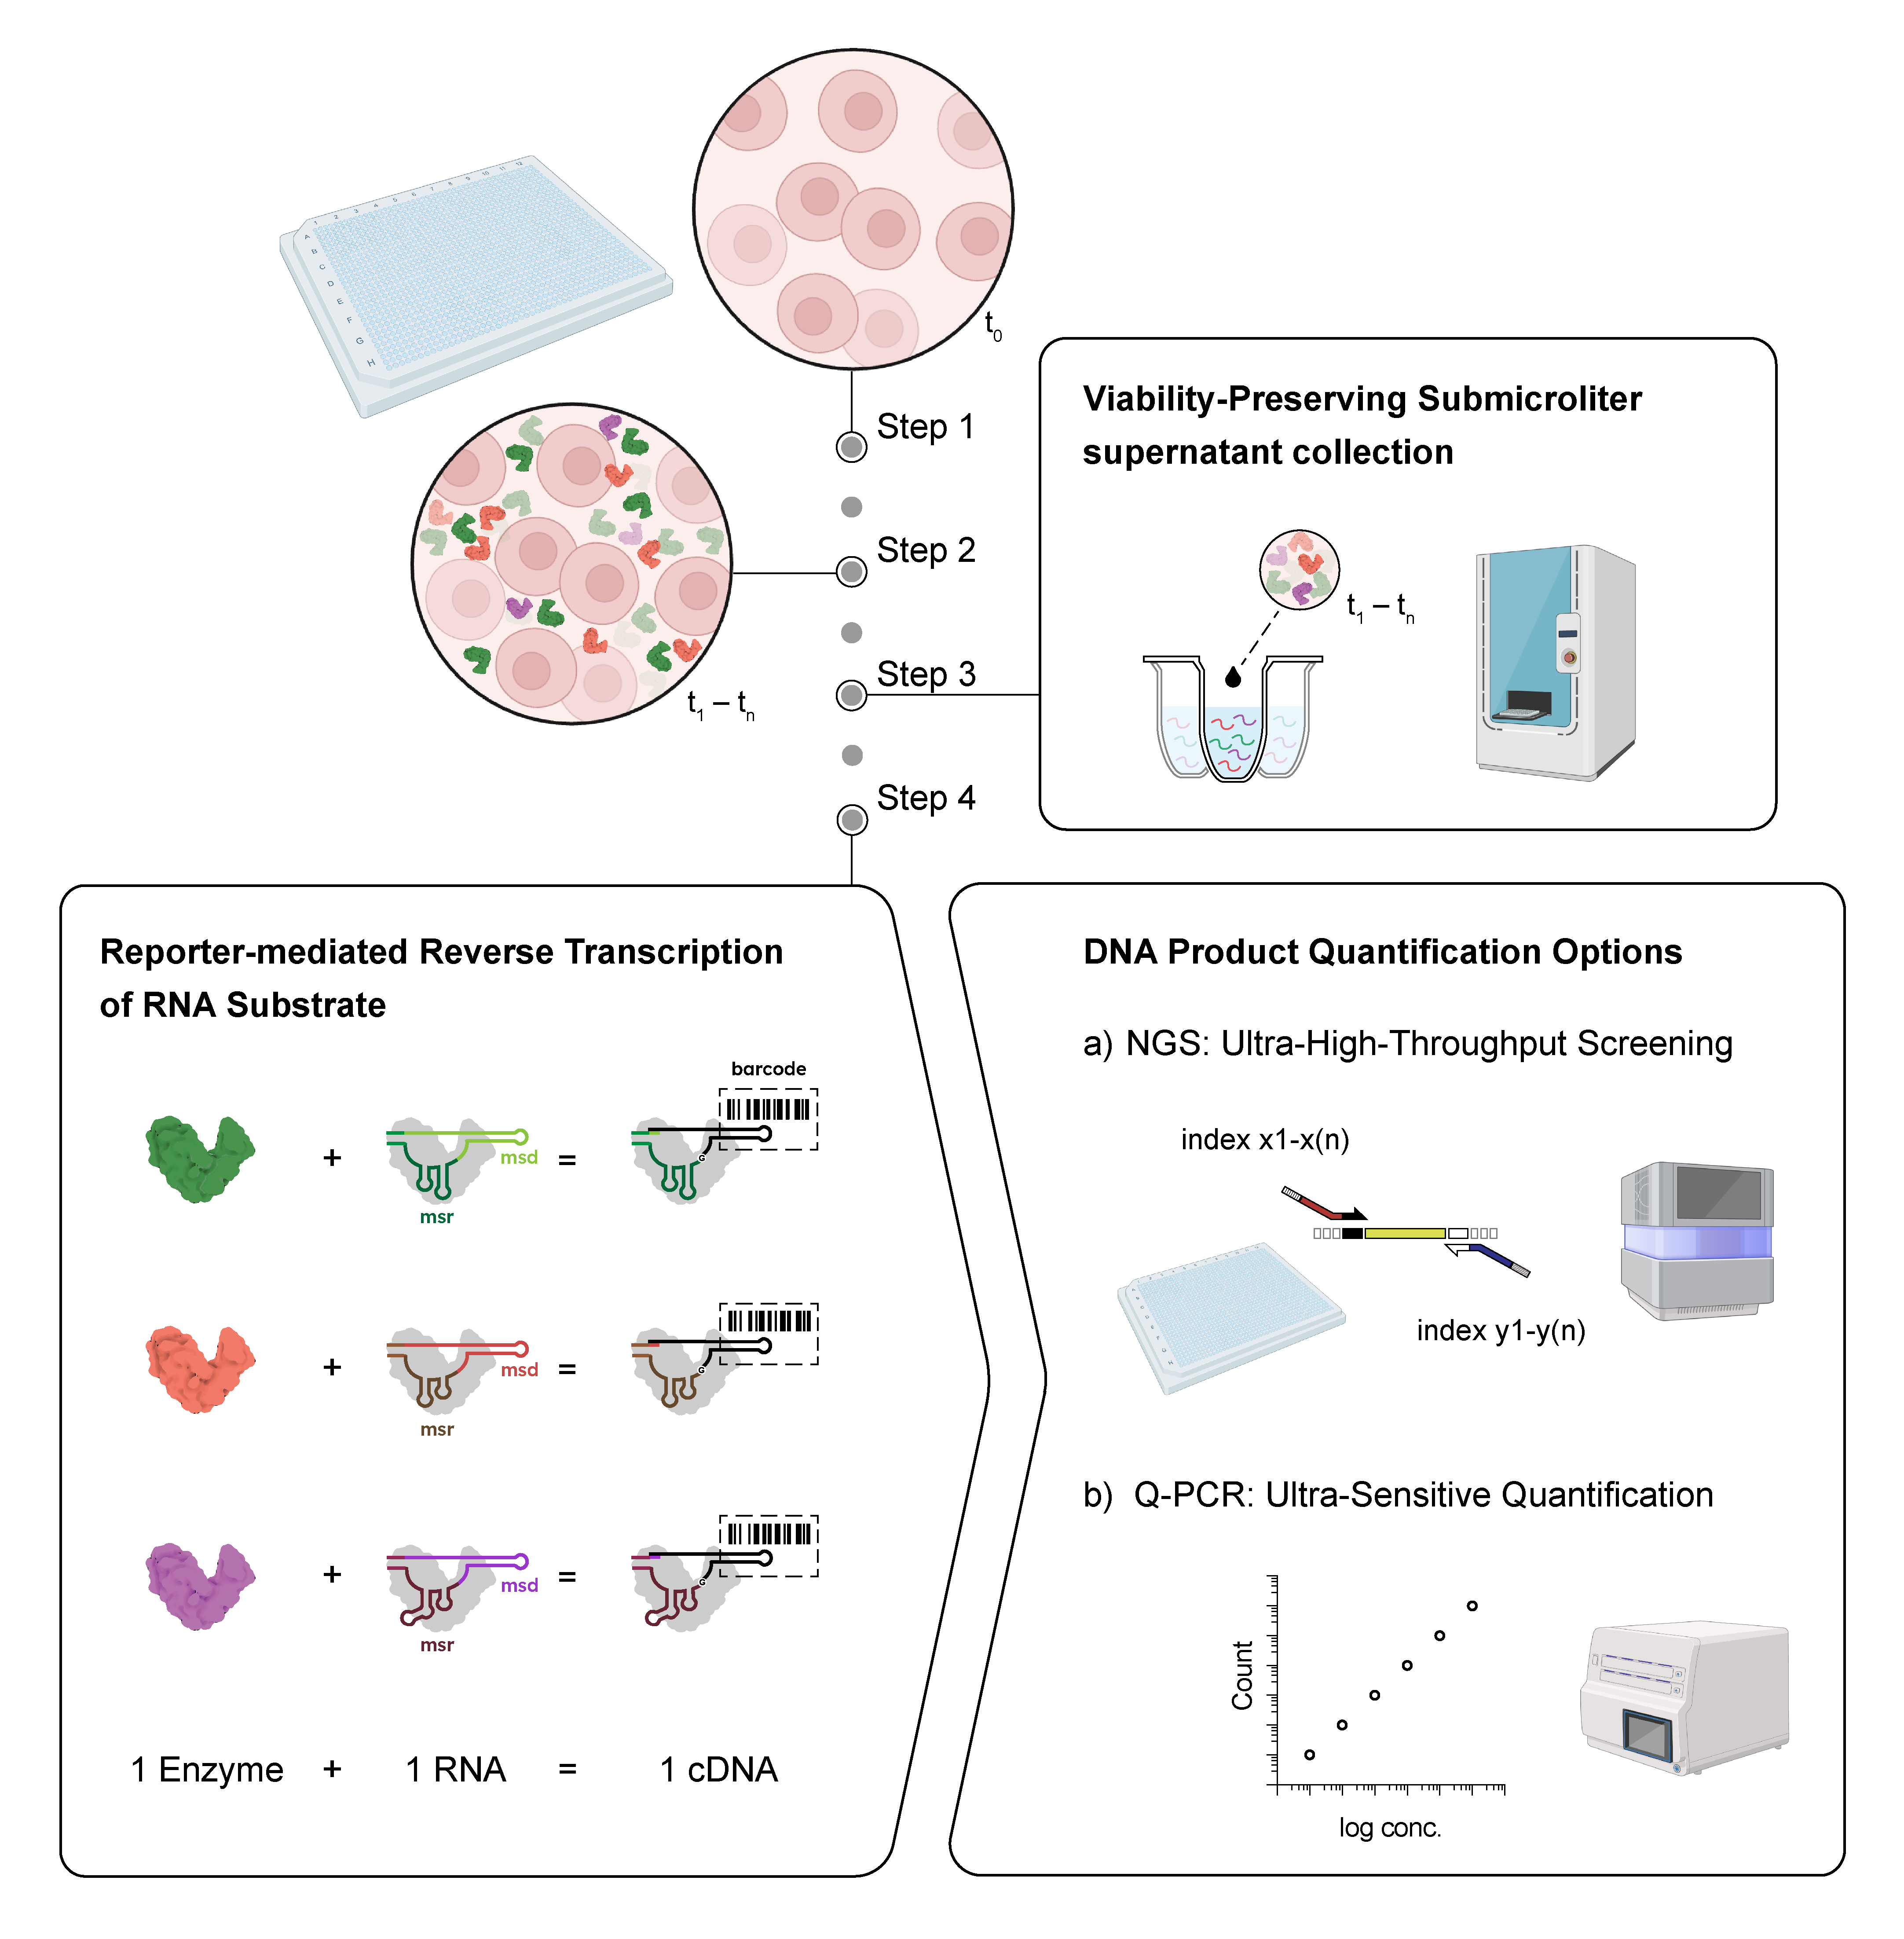
\includegraphics[width=0.75\textwidth]{Graphic_abstract.png}  % Adjust width as needed for smaller image
    \caption{TBD.}
    \label{fig:retron_at_HIL}
\end{figure}


At the Health Innovation Lab, we repurpose retron RTs beyond their established
roles in genome editing and molecular recording, exploiting their enzymatic
activity as a quantitative readout. Our approach reframes the retron not as a
genome-modifying tool but as a \textit{secreted enzymatic reporter}: an
engineered RT that, upon secretion from mammalian cells, remains catalytically
active in the extracellular milieu and reverse-transcribes its cognate ncRNA
into a defined single-stranded DNA product. Three properties of the retron
architecture follow directly from the features described above. Because each RT
recognises only its own ncRNA \cite{shimamoto1993,buffington2025}, distinct
RT--ncRNA pairs can operate orthogonally within the same sample. Because the
\textit{msd} region tolerates synthetic sequence insertion
\cite{simon2019,crawford2025}, each reporter can be encoded with a unique DNA
barcode flanked by common primer-binding sites. And because the enzyme remains
associated with its product after synthesis, the reaction is self-limiting
\cite{inouye1989,shimamoto1993}: with substrate in excess, product abundance
reports the number of secreted enzyme molecules rather than the interval over
which they acted, which removes the sensitivity to substrate-addition and
read-timing differences that accumulates across a microplate. A further
consequence is that the ncRNA is supplied only at the point of analysis, so no
single-stranded DNA is ever synthesised intracellularly. Together these convert
a biological signal into an amplifiable, sequenceable nucleic acid output --- an
inherently multiplexable readout that circumvents the substrate and detection
conflicts limiting conventional secreted enzyme reporters.

To establish feasibility, we designed a secreted dual-reporter fusion protein
pairing a bacterial retron RT domain with NanoLuc, enabling direct benchmarking
against a state-of-the-art secreted reporter within a single construct
\cite{hall2012} (\cref{fig:Prelim}A). Expressed in HEK293T cells, the fusion was
efficiently exported and both domains were active in unprocessed supernatant:
NanoLuc luminescence and retron-generated cDNA barcodes each scaled linearly
with sample volume, with retron activity showing sensitivity comparable to
NanoLuc and quantifiable at sub-microlitre volumes (\cref{fig:Prelim}B,C).
Screening a panel of retron and retron-like RTs identified variants differing in
secretion efficiency and normalised activity (\cref{fig:Prelim}A,B), and
substrate titration confirmed that reporter output tracks substrate availability
while preserving linearity under substrate-limited conditions
(\cref{fig:Prelim}D). Critically, orthogonality holds in practice: when two
retrons were assayed together in the presence of both substrates, cross-activity
fell below the limit of quantitation and each titration curve was unaffected by
the other reporter (\cref{fig:Prelim}E,F) --- the core requirement for
multiplexed detection from a single supernatant sample.

% At the Health Innovation Lab, we repurpose retron RTs beyond their established roles in genome editing and molecular recording, exploiting their enzymatic activity as a quantitative readout. Our approach reframes the retron not as a genome-modifying tool but as a \textit{secreted enzymatic reporter}: an engineered RT that, upon secretion from mammalian cells, remains catalytically active in the extracellular milieu and reverse-transcribes its cognate ncRNA into a defined single-stranded DNA product. Because each retron RT recognizes only its own ncRNA structure, distinct RT–ncRNA pairs can operate orthogonally within the same sample, and because the msd region tolerates synthetic sequence insertions, each reporter can be encoded with a unique DNA barcode flanked by common primer-binding sites. This converts a biological signal into an amplifiable, sequenceable nucleic acid output—an inherently multiplexable readout that circumvents the substrate and detection conflicts limiting conventional secreted enzyme reporters.

% To establish feasibility, we designed a secreted dual-reporter fusion protein pairing a bacterial retron RT domain with NanoLuc, enabling direct benchmarking against a state-of-the-art secreted reporter within a single construct (\cref{fig:placeholder}A). Expressed in HEK293T cells, the fusion was efficiently exported, and both domains were active in unprocessed supernatant: NanoLuc luminescence and retron-generated cDNA barcodes each scaled linearly with sample volume, with retron activity showing sensitivity comparable to NanoLuc and quantifiable at sub-microliter volumes (\cref{fig:placeholder}B; \cref{fig:Prelim}C). Screening a panel of retron/retron-like RTs identified variants that differ in secretion efficiency and normalized activity (\cref{fig:Prelim}A,B), and substrate titration confirmed that reporter output tracks substrate availability while preserving linearity under substrate-limited conditions (\cref{fig:Prelim}D). Critically, we demonstrated orthogonality: when two retrons were assayed together in the presence of both substrates, cross-activity fell below the limit of quantitation and each titration curve was unaffected by the other reporter (\cref{fig:Prelim}E,F), establishing the core requirement for true multiplexed detection from a single supernatant sample.

